%!TEX root = JakubJedryszek2014.tex

\cleardoublepage

\chapter{Verification}
\label{verification}

\begin{chapquote}{\textit{Leonardo da Vinci}}
``It had long since come to my attention that people of accomplishment rarely sat back and let things happen to them. They went out and happened to things.''
\end{chapquote}

The goal of verification process presented in this chapter is to check for run-time errors and show by example how to fix them with the SPARK verification tools. In the future, the same strategy can be used for verification of requirements specified by BLESS annexes in AADL models. As a reminder to the reader, the SPARK 2005 has been identified (as opposed to SPARK 2014, which is still under development) as the most appropriate and capable for the development and verification needs of this thesis work (at the time when this thesis has been written).

The strategy for Software Verification using SPARK 2005 tools is as follows \cite{Barnes:Book}. First, Examiner generates Verification Conditions (VCs) and Dead Path Conjectures (DPCs). Some VCs that can be discharged by simple rewriting are also simplify and discharged by Examiner. Next, SPARKSimp runs Simplifier to simplify and discharge some (or all) VCs that were not discharged by Examiner. SPARKSimp also runs ZombieScope to analyze DPCs and ViCToR to discharge VCs (not discharged by Examiner nor Simplifier) with SMT Solver technology. To provide a summary of verification results, a POGS report is generated. To this standard SPARK 2005 tool chain, Bakar Kiasan symbolic execution tools (developed by the Kansas State University SAnToS research group) has been added. Specifically, when not all Verification Conditions are discharged, analysis continues with Bakar Kiasan. After fixes are made with Kiasan help, Examiner and SPARKSimp tools are run again to confirm correctness. This approach is presented in the Figure \ref{figure:sparkverificationstrategy}. Detailed overview of SPARK verification tools can be found in chapter 12 of SPARK book \cite{Barnes:Book}.

\begin{figure}[ht]%t=top, b=bottom, h=here
    \begin{center}
        
\includegraphics[width=1.0\textwidth]{figures/spark-verification.png}        
    \end{center}
    \caption{Applied Verification strategy}
    \label{figure:sparkverificationstrategy}
\end{figure}

\section{Verification of Implemented PCA Pump Prototype}
\label{verification:prototype}

During PCA Pump Prototype implementation, program syntax was regularly checked with SPARK Examiner. The complete, manually implemented prototype, which can be found in Appendix \ref{Appendix:pca_ravenscar}, was verified with the strategy given at the beginning of this chapter (excluding Bakar Kiasan, which does not handle Ravenscar programs). Thus SPARK Examiner, SPARKSimp (Simplifier, ZombieScope and ViCToR) and POGS were used. Package \lstinline{Pca_Engine} was excluded from verification, using \lstinline{--# hide} annotation, because it contains Ada code, which is non-valid SPARK. The result of this analysis, in the form of a POGS report summary, is presented in the Figure \ref{listing:pca_ravenscar:pogs}. The full report can be found in Appendix \ref{Appendix:pca_ravenscar:pogs}.

The POGS report shows that 30\% (90) of VCs were discharged by Examiner and 61\% (183) by Simplifier. There are 29 undischarged VCs. All of them are caused by possible overflows and array index out of bounds. In addition to VCs, DPCs were generated and 32 dead paths were found. Some undischarged VCs and dead paths come from procedures responsible for maximum dose monitoring. As mentioned in chapter \ref{background:sparkverification:sireum}, Bakar Kiasan does not support Ravenscar profile. For the demonstration purpose, sequential module for dose monitoring has been created in order to analyze undischarged VCs. Verification process of this module is described in Section \ref{verification:pcapump:monitoring}.

\begin{figure}
\singlespacing
\begin{lstlisting}[frame=single, gobble=0]
Summary:

Proof strategies used by subprograms
-------------------------------------------------------------------------
Total subprograms with at least one VC proved by examiner:             15
Total subprograms with at least one VC proved by simplifier:           20
Total subprograms with at least one VC proved by contradiction:         0
Total subprograms with at least one VC proved with user proof rule:     0
Total subprograms with at least one VC proved by Victor:                0
Total subprograms with at least one VC proved by Riposte:               0
Total subprograms with at least one VC proved using checker:            0
Total subprograms with at least one VC discharged by review:            0

Maximum extent of strategies used for fully proved subprograms:
-------------------------------------------------------------------------
Total subprograms with proof completed by examiner:                     0
Total subprograms with proof completed by simplifier:                  14
Total subprograms with proof completed with user defined rules:         0
Total subprograms with proof completed by Victor:                       0
Total subprograms with proof completed by Riposte:                      0
Total subprograms with proof completed by checker:                      0
Total subprograms with VCs discharged by review:                        0

Overall subprogram summary:
-------------------------------------------------------------------------
Total subprograms fully proved:                                        14
Total subprograms with at least one undischarged VC:                    8  <<<
Total subprograms with at least one false VC:                           0
                                                                    -----
Total subprograms for which VCs have been generated:                   22


ZombieScope Summary:
-------------------------------------------------------------------------
Total subprograms for which DPCs have been generated:                  22
Total number subprograms with dead paths found:                         3
Total number of dead paths found:                                      32


VC summary:
-------------------------------------------------------------------------
Note: (User) denotes where the Simplifier has proved VCs using one or
      more user-defined proof rules.

Total VCs by type:
------------------
                    Total   Examiner Simplifier    Undisc.
Assert/Post            93         80         12          1
Precondition           12          0         12          0
Check stmnt.            0          0          0          0
Runtime check         187          0        159         28
Refinem. VCs           10         10          0          0
Inherit. VCs            0          0          0          0
==========================================================
Totals:               302         90        183         29 <<<
%Totals:                         30%        61%        10%

===================== End of Semantic Analysis Summary ========================
\end{lstlisting}
\doublespacing
\caption{Summary of POGS report for PCA Pump prototype}
\label{listing:pca_ravenscar:pogs}
\end{figure}



\section{Monitoring Dosed Amount}
\label{verification:pcapump:monitoring}

This section is a case study of verifying the SPARK module responsible for tracking the dosed amount of drug. The module was created in the sequential SPARK 2005 profile, based on implemented PCA prototype presented in Appendix \ref{Appendix:pca_ravenscar}. The isolated module implementation is presented in the Figure \ref{listing:pcapump_dosemonitor}.

\begin{figure}
\singlespacing
\begin{lstlisting}[language=ada, frame=single, gobble=0]
package Pca_Pump
--# own Dosed;
--#     Dose_Volume;
--# initializes Dosed,
--#             Dose_Volume;
is
    subtype Integer_Array_Index is Integer range 1 .. 60*60;
    type Integer_Array is array (Integer_Array_Index) of Integer;

    procedure Increase_Dosed;
    --# global in out Dosed;
    --#        in Dose_Volume;
    --# derives Dosed from Dosed, Dose_Volume;

    function Read_Dosed return Integer;
    --# global in Dosed;

    procedure Move_Dosed;
    --# global in out Dosed;
    --# derives Dosed from Dosed;

end Pca_Pump;

package body Pca_Pump
is
    Dosed : Integer_Array := Integer_Array'(others => 0);
    Dose_Volume : Integer := 1;

    procedure Increase_Dosed
    is
    begin
        Dosed(Integer_Array_Index'Last) := Dosed(Integer_Array_Index'Last) + Dose_Volume;
    end Increase_Dosed;

    function Read_Dosed return Integer
    is
        Result : Integer := 0;
    begin
        for I in Integer_Array_Index loop
            --# assert I > 1 -> Result >= Dosed(I-1);
            Result := Result + Dosed(I);
        end loop;
        return Result;
    end Read_Dosed;

    procedure Move_Dosed
    is
    begin
        for I in Integer_Array_Index range 1 .. Integer_Array_Index'Last-1 loop
            --# assert I > 1 -> Dosed(I-1) = Dosed(I);
            Dosed(I) := Dosed(I+1);
        end loop;
        Dosed(Integer_Array_Index'Last) := 0;
    end Move_Dosed;

end Pca_Pump;
\end{lstlisting}
\doublespacing
\caption{Dose monitor module specification}
\label{listing:pcapump_dosemonitor}
\end{figure}

Verification strategy is based on Figure \ref{figure:sparkverificationstrategy}. First, the program is verified with Examiner, SPARKSimp (Simplifier, ZombieScope and Victor). A Verification report is generated by POGS. In case of any unfinished verification steps, verification is continued with Bakar Kiasan, which gives more user friendly experience that POGS report and generated VC files. It may be preferable to use Bakar Kiasan first, but in this thesis SPARK 2005 verification tools created by AdaCore and Altran were used first to indicate not verified code.

First verification report generated by POGS is presented in the Figure \ref{listing:pcapump_dosemonitor_pogs}. It indicates presence of three undischarged (not proved) VCs.

\begin{figure}
\singlespacing
\begin{lstlisting}[frame=single, gobble=0]
Summary:

Proof strategies used by subprograms
-------------------------------------------------------------------------
Total subprograms with at least one VC proved by examiner:              2
Total subprograms with at least one VC proved by simplifier:            2
Total subprograms with at least one VC proved by contradiction:         0
Total subprograms with at least one VC proved with user proof rule:     0
Total subprograms with at least one VC proved by Victor:                0
Total subprograms with at least one VC proved by Riposte:               0
Total subprograms with at least one VC proved using checker:            0
Total subprograms with at least one VC discharged by review:            0

Maximum extent of strategies used for fully proved subprograms:
-------------------------------------------------------------------------
Total subprograms with proof completed by examiner:                     0
Total subprograms with proof completed by simplifier:                   1
Total subprograms with proof completed with user defined rules:         0
Total subprograms with proof completed by Victor:                       0
Total subprograms with proof completed by Riposte:                      0
Total subprograms with proof completed by checker:                      0
Total subprograms with VCs discharged by review:                        0

Overall subprogram summary:
-------------------------------------------------------------------------
Total subprograms fully proved:                                         1
Total subprograms with at least one undischarged VC:                    2  <<<
Total subprograms with at least one false VC:                           0
                                                                    -----
Total subprograms for which VCs have been generated:                    3


ZombieScope Summary:
-------------------------------------------------------------------------
Total subprograms for which DPCs have been generated:                   3
Total number subprograms with dead paths found:                         1
Total number of dead paths found:                                       1


VC summary:
-------------------------------------------------------------------------
Note: (User) denotes where the Simplifier has proved VCs using one or
      more user-defined proof rules.

Total VCs by type:
------------------
                    Total   Examiner Simplifier    Undisc.
Assert/Post             8          3          4          1
Precondition            0          0          0          0
Check stmnt.            0          0          0          0
Runtime check           7          0          5          2
Refinem. VCs            0          0          0          0
Inherit. VCs            0          0          0          0
==========================================================
Totals:                15          3          9          3 <<<
%Totals:                         20%        60%        20%

===================== End of Semantic Analysis Summary ========================
\end{lstlisting}
\doublespacing
\caption{POGS report}
\label{listing:pcapump_dosemonitor_pogs}
\end{figure}

Next, according to verification strategy, instead of VC analysis Bakar Kiasan was run to find out why program is not fully verified. Kiasan report is presented in the Figure \ref{figure:sparkverification:kiasanreport1}.

\begin{figure}[ht]%t=top, b=bottom, h=here
    \begin{center}
        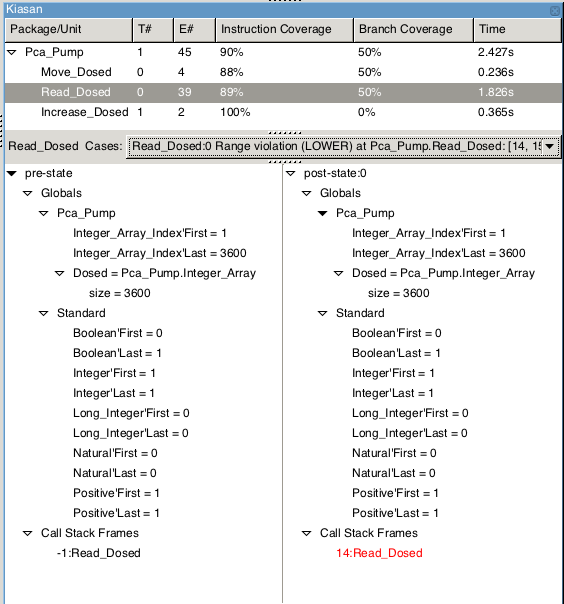
\includegraphics[width=0.8\textwidth]{figures/pca-pump-verification-step1.png}        
    \end{center}    
    \caption{Bakar Kiasan verification report}
    \label{figure:sparkverification:kiasanreport1}
\end{figure}

The first issue we can notice is problem with data types' ranges indicated by Exception cases, e.g., \lstinline{Read_Dosed:0 Range violation (LOWER) at Pca_Pump.Read_Dosed:[14,15]} (presented in Figure \ref{figure:sparkverification:kiasanreport1}). To solve it (in SPARK 2005) configuration file \lstinline{Standard.ads} (presented in Figure \ref{figure:sparkverification:config}), which specifies \lstinline{Integer} type range, was created. This is information for verification tools, which may helps in verification. The Kiasan verification report generated after that is presented in Figure \ref{figure:sparkverification:kiasanreport2}. The number of errors is reduced, but now there is possible overflow violation indicated e.g. by Exception case 0 for \lstinline{Increase_Dosed} procedure: \lstinline{Arithmetic overflow violation (LOWER) at Pca_Pump.Increase_Dosed: [9,90]} (presented in Figure \ref{figure:sparkverification:kiasanreport2}).

\begin{figure}
\singlespacing
\begin{lstlisting}[frame=single, gobble=0]
package Standard is

    type Integer is range -2**31 .. 2**31-1;

end Standard;
\end{lstlisting}
\doublespacing
\caption{Configuration file for Bakar Kiasan}
\label{figure:sparkverification:config}
\end{figure}

\begin{figure}[ht]%t=top, b=bottom, h=here
    \begin{center}
        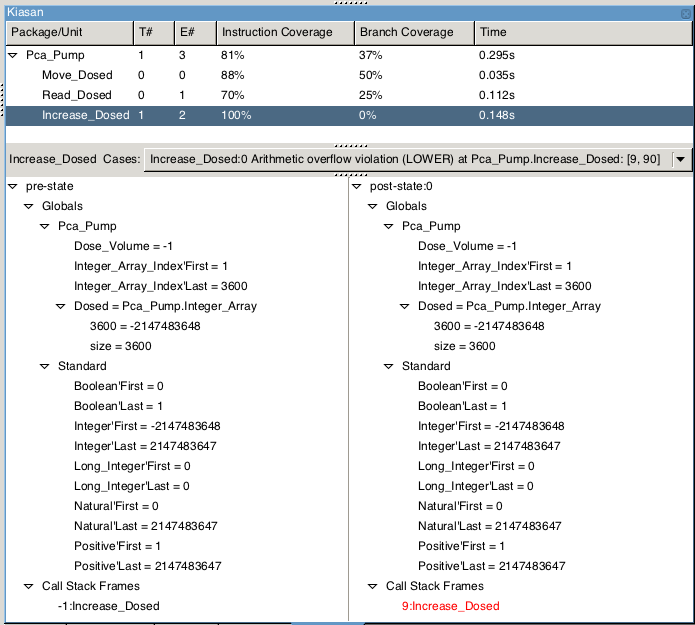
\includegraphics[width=0.8\textwidth]{figures/pca-pump-verification-step2.png}        
    \end{center}
    \caption{Bakar Kiasan verification report, second run}
    \label{figure:sparkverification:kiasanreport2}
\end{figure}

From functional perspective, negative values are not needed it this case, thus new type \lstinline{Drug_Volume} type was created. \lstinline{Integer_Array} type was renamed to \lstinline{Doses_Array} and its type was changed to \lstinline{Drug_Volume}. Result of Kiasan analysis after this change is presented in Figure \ref{figure:sparkverification:kiasanreport3}.

\begin{figure}[ht]%t=top, b=bottom, h=here
    \begin{center}
        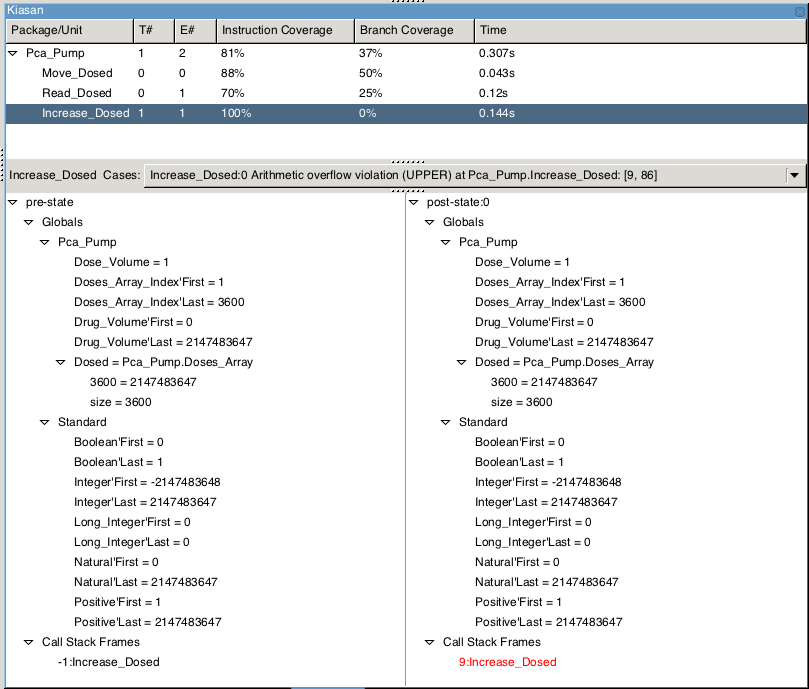
\includegraphics[width=0.8\textwidth]{figures/pca-pump-verification-step3.png}        
    \end{center}
    \caption{Bakar Kiasan verification report, third run}
    \label{figure:sparkverification:kiasanreport3}
\end{figure}

This change eliminated lower overflow, because now negative value cannot be added to any array element. Only upper overflow in \lstinline{Increase_Dosed} procedure error was left. The fix for this is the introduction of precondition for \lstinline{Increase_Dosed}: \lstinline{--# pre Read_Dosed(Dosed) <= Drug_Volume'Last - Dose_Volume;}. Addition of this contract caused semantic error (detected by Examiner): \lstinline{The identifier Read_Dosed is either undeclared or not visible at this point}. This error is caused by the definition of \lstinline{Increase_Dosed} procedure before \lstinline{Read_Dosed} procedure. To fix, this \lstinline{Read_Dosed} procedure was moved before \lstinline{Increase_Dosed}. However, after that Examiner returned different error: \lstinline{Binary operator is not declared for types Drug_Volume and Dose_Volume__type}. To make the operator visible, \lstinline{Dose_Volume} type has to be declared in \lstinline{--# own} annotation: \lstinline{--# Dose_Volume : Drug_Volume;}. After these fixes, Kiasan analysis has be run again. The result is depicted in the Figure \ref{figure:sparkverification:kiasanreport4}.

\begin{figure}[ht]%t=top, b=bottom, h=here
    \begin{center}
        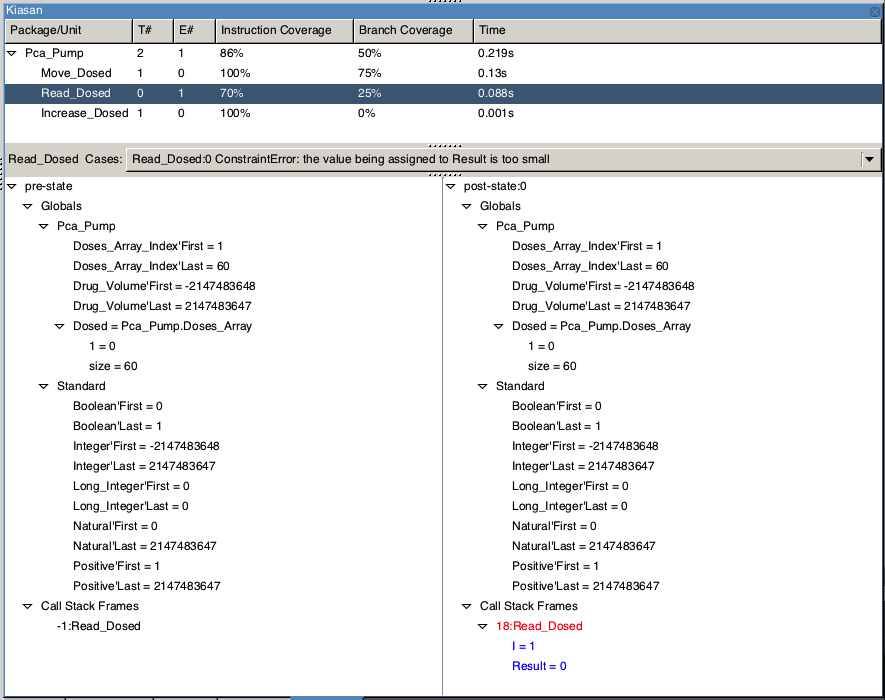
\includegraphics[width=0.8\textwidth]{figures/pca-pump-verification-step4.png}
    \end{center}
    \caption{Bakar Kiasan verification report, forth run}
    \label{figure:sparkverification:kiasanreport4}
\end{figure}

There were no error cases in the \lstinline{Move_Dosed} and the \lstinline{Increase_Dosed} procedures. The error case in \lstinline{Read_Dosed} is shown in Figure \ref{figure:sparkverification:kiasanreport4}. It is \lstinline{ConstraintError: the value being assigned to Result is too small}. This error is not very informative. After investigation and talks with the Kiasan Developer, it was determined that there is a bug in Kiasan v1 (for SPARK 2005). More precisely: in handling overflows. For the purpose of verification, \lstinline{Drug_Volume} type range was changed to $0 - (2^{15} - 1)$. This will give range up to around 1000000, which is sufficient even if calculations are made in micro liters (as it is in case of PCA pump prototype implementation). 1000000 micro liters is 1000 ml, which is 1 liter. This is an extreme amount of drug in case of PCA pump, according to Requirements Document \cite{PcaReq}. The bug with type ranges is fixed in Kiasan v2 (for SPARK 2014).

Another problem was the size of \lstinline{Dosed} array (3600 elements). Kiasan allows the developer to configure the array bound and loop bound. Both had to be increased (from default 10). Another thing was computational complexity. For 3600 elements, state space grows exponentially and it takes a lot of time to analyze it. Thus, for verification purposes, array size was changed to 60 elements along with change to array bounds and loop bounds, also to 60.

After rerunning Kiasan, there is valid test case for \lstinline{Read_Dose}, but there are also 59 Exception cases: \lstinline{Range violation (UPPER)}, which means possible overflow. One way of fix this problem, was to add an \lstinline{--# assume} annotation to loop in function body, stating that every sum operation in the loop will not cause overflow, but Kiasan v1 does not support \lstinline{assume} annotations. Another way was to add precondition that ensures, that the sum of elements is lower than \lstinline{Drug_Volume'Last}. SPARK does not provide simple library for summing an array (like the Contracts language for Java provides). Thus, this function had to be implemented. Its implementation is the same as \lstinline{Read_Dosed}. It sums all elements of array. The \lstinline{Sum} function specification and body is presented in the Figure \ref{listing:sum_function}.

\begin{figure}
\singlespacing
\begin{lstlisting}[language=ada, frame=single, gobble=0]
function Sum(Arr : Doses_Array) return Drug_Volume;

function Sum(Arr : Doses_Array) return Drug_Volume
is
    Result : Drug_Volume := 0;
begin
    for I in Doses_Array_Index loop
        --# assert true;
        Result := Result + Arr(I);
    end loop;
    return Result;
end Sum;
\end{lstlisting}
\doublespacing
\caption{Sum function for summing all elements of array}
\label{listing:sum_function}
\end{figure}

After rerunning Kiasan, only valid test cases were found, which is depicted in the Figure \ref{figure:sparkverification:kiasanreport5}.

\begin{figure}[ht]%t=top, b=bottom, h=here
    \begin{center}
        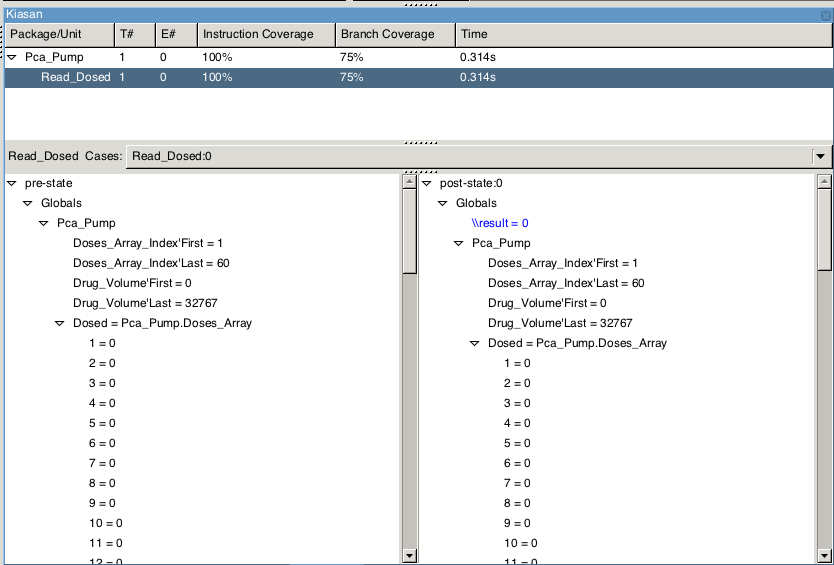
\includegraphics[width=0.8\textwidth]{figures/pca-pump-verification-step5.png}        
    \end{center}
    \caption{Bakar Kiasan verification report, fifth run}
    \label{figure:sparkverification:kiasanreport5}
\end{figure}

The last thing which was improved by code contracts is checking if \lstinline{Move_Dosed} procedure works as expected. In that purpose three postconditions were added (Figure \ref{listing:postconditions_added_to_move_dosed}). First checks if the last element is equal to 0. Second and third checks two possible scenarios: 
\begin{itemize}
    \item before running procedure, the first element is equal to 0: amount of dosed drug in last hour will not change after Dosed procedure execution
    \item the first element is greater than 0: after Dosed procedure execution, the amount of drug dosed in last hour will decrease, because first element value will no longer be in last hour range
\end{itemize}

\begin{figure}
\singlespacing
\begin{lstlisting}[language=ada, frame=single, gobble=0]
--# post Dosed(Doses_Array_Index'Last) = 0 
--#      and (Dosed~(Doses_Array_Index'First)=0 -> Read_Dosed(Dosed~) = Read_Dosed(Dosed))
--#      and (Dosed~(Doses_Array_Index'First)>0 -> Read_Dosed(Dosed~) > Read_Dosed(Dosed));
\end{lstlisting}
\doublespacing
\caption{Postconditions added to \lstinline{Move_Dosed} procedure}
\label{listing:postconditions_added_to_move_dosed}
\end{figure}

After adding these postconditions Kiasan generates 2 test cases to check both mentioned scenarios. There is no error cases, which means that procedure works as expected. 

Another way to validate such requirements is to create AUnit tests. In Section \ref{verification:aunit}, there is an overview of unit tests created to test behavior described above. Furthermore, symbolic execution technique (used by Kiasan) allows to generate AUnit tests automatically, and this feature is under development in Kiasan v2.

To validate changes made, while working with Kiasan, SPARK Examiner and SPARKSimp were rerun again. POGS report is presented in the Figure \ref{listing:pcapump_dosemonitor_pogs3}.

\begin{figure}
\singlespacing
\begin{lstlisting}[frame=single, gobble=0]
VCs for procedure_increase_dosed :
 -----------------------------------------------------------------------------
| #   | From  | To                  | Proved By          | Dead Path | Status |
|-----------------------------------------------------------------------------
| 1   | start | rtc check @ 20      | Undischarged       | Unchecked |   UU   |
| 2   | start |    assert @ finish  | Examiner           | Live      |   EL   |
 -----------------------------------------------------------------------------

VCs for procedure_move_dosed :
 -----------------------------------------------------------------------------
| #   | From  | To                  | Proved By          | Dead Path | Status |
|-----------------------------------------------------------------------------
| 1   | start | rtc check @ 37      | Inference          | Unchecked |   IU   |
| 2   | start | rtc check @ 37      | Inference          | Unchecked |   IU   |
| 3   | start |    assert @ 38      | Inference          | Live      |   IL   |
| 4   | 38    |    assert @ 38      | Inference          | Live      |   IL   |
| 5   | 38    | rtc check @ 39      | Inference          | Unchecked |   IU   |
| 6   | start | rtc check @ 41      | Inference          | Unchecked |   IU   |
| 7   | 38    | rtc check @ 41      | Inference          | Unchecked |   IU   |
| 8   | start |    assert @ finish  | Inference          | Dead      |   ID   |
| 9   | 38    |    assert @ finish  | Undischarged       | Live      |   UL   |
 -----------------------------------------------------------------------------

VCs for function_read_dosed :
 -----------------------------------------------------------------------------
| #   | From  | To                  | Proved By          | Dead Path | Status |
|-----------------------------------------------------------------------------
| 1   | start |    assert @ 28      | Inference          | Live      |   IL   |
| 2   | 28    |    assert @ 28      | Inference          | Live      |   IL   |
| 3   | 28    | rtc check @ 29      | Undischarged       | Unchecked |   UU   |
| 4   | 28    |    assert @ finish  | Inference          | Live      |   IL   |
 -----------------------------------------------------------------------------

VCs for function_sum :
 -----------------------------------------------------------------------------
| #   | From  | To                  | Proved By          | Dead Path | Status |
|-----------------------------------------------------------------------------
| 1   | start |    assert @ 11      | Inference          | Live      |   IL   |
| 2   | 11    |    assert @ 11      | Inference          | Live      |   IL   |
| 3   | 11    | rtc check @ 12      | Undischarged       | Unchecked |   UU   |
| 4   | 11    |    assert @ finish  | Inference          | Live      |   IL   |
 -----------------------------------------------------------------------------

===============================================================================
Summary:

Total VCs by type:
------------------
                    Total   Examiner Simplifier    Undisc.
Assert/Post            11          1          9          1
Precondition            0          0          0          0
Check stmnt.            0          0          0          0
Runtime check           8          0          5          3
Refinem. VCs            0          0          0          0
Inherit. VCs            0          0          0          0
==========================================================
Totals:                19          1         14          4 <<<
%Totals:                          5%        74%        21%
\end{lstlisting}
\doublespacing
\caption{Third POGS report}
\label{listing:pcapump_dosemonitor_pogs3}
\end{figure}

There are 4 undischarged VCs, but total number of generated VCs is 19. In previous run there were only 15. Thus, there are 4 new VCs, and 2 of them are undischarged. The reason is introduction of \lstinline{Sum} function used by all subprograms. This can be confirmed by examining all undischarged VCs: 1st VC in \lstinline{increase_dosed.siv} file (Figure \ref{listing:pcapump_undischarged_vc_increase_dosed}), 9th VC in \lstinline{move_dosed.siv} file (Figure \ref{listing:pcapump_undischarged_vc_move_dosed}), 3rd VC in \lstinline{read_dosed.vcg} file (Figure \ref{listing:pcapump_undischarged_vc_read_dosed}) and 3rd VC in \lstinline{sum.vcg} file (Figure \ref{listing:pcapump_undischarged_vc_sum}). They derived form the subprograms: \lstinline{Increase_Dosed}, \lstinline{Move_Dosed}, \lstinline{Read_Dosed} and \lstinline{Sum} respectively.

\begin{figure}
\singlespacing
\begin{lstlisting}[frame=single, gobble=0]
procedure_increase_dosed_1.
H1:    read_dosed(dosed) <= 32767 - dose_volume .
H2:    for_all(i___1 : integer, 1 <= i___1 and i___1 <= 60 -> 0 <= element(
          dosed, [i___1]) and element(dosed, [i___1]) <= 32767) .
H3:    dose_volume >= 0 .
H4:    dose_volume <= 32767 .
H5:    integer__size >= 0 .
H6:    drug_volume__size >= 0 .
H7:    drug_volume__base__first <= drug_volume__base__last .
H8:    doses_array_index__size >= 0 .
H9:    drug_volume__base__first <= 0 .
H10:   drug_volume__base__last >= 32767 .
       ->
C1:    element(dosed, [60]) + dose_volume <= 32767 .
\end{lstlisting}
\doublespacing
\caption{Undischarged Verification Condition from \lstinline{increase_dosed.siv} file}
\label{listing:pcapump_undischarged_vc_increase_dosed}
\end{figure}

\begin{figure}
\singlespacing
\begin{lstlisting}[frame=single, gobble=0]
procedure_move_dosed_9.
H1:    element(dosed, [58]) = element(dosed, [59]) .
H2:    for_all(i___1 : integer, 1 <= i___1 and i___1 <= 60 -> 0 <= element(
          dosed, [i___1]) and element(dosed, [i___1]) <= 32767) .
H3:    element(dosed, [60]) >= 0 .
H4:    element(dosed, [60]) <= 32767 .
H5:    integer__size >= 0 .
H6:    drug_volume__size >= 0 .
H7:    drug_volume__base__first <= drug_volume__base__last .
H8:    doses_array_index__size >= 0 .
H9:    drug_volume__base__first <= 0 .
H10:   drug_volume__base__last >= 32767 .
       ->
C1:    element(dosed~, [1]) = 0 -> read_dosed(dosed~) = read_dosed(update(
          update(dosed, [59], element(dosed, [60])), [60], 0)) .
C2:    element(dosed~, [1]) > 0 -> read_dosed(dosed~) > read_dosed(update(
          update(dosed, [59], element(dosed, [60])), [60], 0)) .
\end{lstlisting}
\doublespacing
\caption{Undischarged Verification Condition from \lstinline{move_dosed.siv} file}
\label{listing:pcapump_undischarged_vc_move_dosed}
\end{figure}

\begin{figure}
\singlespacing
\begin{lstlisting}[frame=single, gobble=0]
function_read_dosed_3.
H1:    loop__1__i > 1 -> result >= element(dosed, [loop__1__i - 1]) .
H2:    for_all(i___1 : integer, 1 <= i___1 and i___1 <= 60 -> 0 <= element(
          dosed, [i___1]) and element(dosed, [i___1]) <= 32767) .
H3:    sum(dosed) <= 32767 .
H4:    loop__1__i >= 1 .
H5:    loop__1__i <= 60 .
H6:    result >= 0 .
H7:    result <= 32767 .
H8:    integer__size >= 0 .
H9:    drug_volume__size >= 0 .
H10:   drug_volume__base__first <= drug_volume__base__last .
H11:   doses_array_index__size >= 0 .
H12:   drug_volume__base__first <= 0 .
H13:   drug_volume__base__last >= 32767 .
       ->
C1:    result + element(dosed, [loop__1__i]) <= 32767 .
\end{lstlisting}
\doublespacing
\caption{Undischarged Verification Condition from \lstinline{read_dosed.siv} file}
\label{listing:pcapump_undischarged_vc_read_dosed}
\end{figure}

\begin{figure}
\singlespacing
\begin{lstlisting}[frame=single, gobble=0]
function_sum_3.
H1:    for_all(i___1 : integer, 1 <= i___1 and i___1 <= 60 -> 0 <= element(arr, 
          [i___1]) and element(arr, [i___1]) <= 32767) .
H2:    loop__1__i >= 1 .
H3:    loop__1__i <= 60 .
H4:    result >= 0 .
H5:    result <= 32767 .
H6:    integer__size >= 0 .
H7:    drug_volume__size >= 0 .
H8:    drug_volume__base__first <= drug_volume__base__last .
H9:    doses_array_index__size >= 0 .
H10:   drug_volume__base__first <= 0 .
H11:   drug_volume__base__last >= 32767 .
       ->
C1:    result + element(arr, [loop__1__i]) <= 32767 .
\end{lstlisting}
\doublespacing
\caption{Undischarged Verification Condition from \lstinline{sum.siv} file}
\label{listing:pcapump_undischarged_vc_sum}
\end{figure}

In \lstinline{Move_Dosed} procedure, the SPARK tools cannot prove the implications in post conditions. Fortunately, it is already proved by Bakar Kiasan. The problem in \lstinline{Increase_Dosed}, \lstinline{Read_Dosed} and \lstinline{Sum} is the same. The SPARK tools cannot verify, that adding \lstinline{Result} and some element of \lstinline{Dosed} array will not cause overflow. Bakar Kiasan can prove correctness of \lstinline{Increase_Dosed} and \lstinline{Read_Dosed}. However only, with assumption that \lstinline{Sum} is correct. Four exception cases indicating possible overflow are generated. Thus, the only way to discharge the verification obligation of this module is to assume that the proof function \lstinline{Sum} is correct.

In procedure \lstinline{Move_Dosed}, there is one dead path found. POGS report gives only information where dead path exists, but not in which circumstances. The information about conditions, in which dead path occurs is stored in \lstinline{.dpc} file. The file path to concrete file is given in the POGS report just before summary table for procedure \lstinline{Move_Dosed}. In this case it is \lstinline{move_dosed.dpc} file. Figure \ref{listing:pcapump_dosemonitor_pogs3} presents truncated POGS report, but as an example, full POGS report of implemented PCA prototype can be found in Appendix \ref{Appendix:pca_ravenscar:pogs} (e.g. see line 50, which contains DPC analysis for \lstinline{Start_Pumping} procedure). 

The relevant fragment, which applies to the found dead path is presented in the Figure \ref{listing:pcapump_dosemonitor:dead_path}. It is a list of hypothesis, in which hypothesis 10 (H10) states that number of elements in \lstinline{Doses_Array} is 1 or less. In this case (or more precisely: in this path), \lstinline{for loop} will not be visited. \lstinline{Doses_Array} has always 60 elements, thus this path is impossible (dead). It does not mean something bad, because dead path indicate possible issues. In this case it is not issue. It is expected behavior.

\begin{figure}
\singlespacing
\begin{lstlisting}[frame=single, gobble=0]
procedure_move_dosed_8.
H1:    for_all(i___1: integer, ((i___1 >= doses_array_index__first) and (
           i___1 <= doses_array_index__last)) -> ((element(
           dosed, [i___1]) >= drug_volume__first) and (element(
           dosed, [i___1]) <= drug_volume__last))) .
H2:    doses_array_index__last - 1 >= integer__first .
H3:    doses_array_index__last - 1 <= integer__last .
H4:    doses_array_index__last - 1 >= integer__base__first .
H5:    doses_array_index__last - 1 <= integer__base__last .
H6:    doses_array_index__first >= integer__first .
H7:    doses_array_index__first <= integer__last .
H8:    (doses_array_index__first <= doses_array_index__last - 1) -> ((
           doses_array_index__last - 1 >= doses_array_index__first) and (
           doses_array_index__last - 1 <= doses_array_index__last)) .
H9:    (doses_array_index__first <= doses_array_index__last - 1) -> ((
           doses_array_index__first >= doses_array_index__first) and (
           doses_array_index__first <= doses_array_index__last)) .
H10:   not (doses_array_index__first <= doses_array_index__last - 1) .
H11:   0 >= drug_volume__first .
H12:   0 <= drug_volume__last .
H13:   doses_array_index__last >= doses_array_index__first .
H14:   doses_array_index__last <= doses_array_index__last .
        ->
C1:    false .
\end{lstlisting}
\doublespacing
\caption{Dead path in \lstinline{Move_Dosed} procedure}
\label{listing:pcapump_dosemonitor:dead_path}
\end{figure}

The complete code of the module for dose monitoring, after changes described above, is presented in Figures \ref{listing:pcapump_dosemonitor:spark2005_spec} and \ref{listing:pcapump_dosemonitor:spark2005_body}.

\begin{figure}
\singlespacing
\begin{lstlisting}[frame=single, gobble=0]
package Pca_Pump
--# own Dosed : Doses_Array;
--#     Dose_Volume : Drug_Volume;
--# initializes Dosed,
--#             Dose_Volume;
is
    type Drug_Volume is range 0 .. 2**15-1;

    subtype Doses_Array_Index is Positive range 1 .. 60;
    type Doses_Array is array (Doses_Array_Index) of Drug_Volume;

    function Sum(Arr : Doses_Array) return Drug_Volume;

    function Read_Dosed return Drug_Volume;
    --# global in Dosed;
    --# pre Sum(Dosed) <= Drug_Volume'Last;

    procedure Increase_Dosed;
    --# global in out Dosed;
    --#        in Dose_Volume;
    --# derives Dosed from Dosed, Dose_Volume;
    --# pre Read_Dosed(Dosed) <= Drug_Volume'Last - Dose_Volume;

    procedure Move_Dosed;
    --# global in out Dosed;
    --# derives Dosed from Dosed;
    --# post Dosed(Doses_Array_Index'Last) = 0
    --#      and (Dosed~(Doses_Array_Index'First)=0 -> Read_Dosed(Dosed~) = Read_Dosed(Dosed))
    --#      and (Dosed~(Doses_Array_Index'First)>0 -> Read_Dosed(Dosed~) > Read_Dosed(Dosed));

end Pca_Pump;
\end{lstlisting}
\doublespacing
\caption{Dose monitoring module after changes: package specification}
\label{listing:pcapump_dosemonitor:spark2005_spec}
\end{figure}

\begin{figure}
\singlespacing
\begin{lstlisting}[frame=single, gobble=0]
package body Pca_Pump
is
    Dosed : Doses_Array := Doses_Array'(others => 0);
    Dose_Volume : Drug_Volume := 1;

    function Sum(Arr : Doses_Array) return Drug_Volume
    is
        Result : Drug_Volume := 0;
    begin
        for I in Doses_Array_Index loop
            --# assert true;
            Result := Result + Arr(I);
        end loop;
        return Result;
    end Sum;

    procedure Increase_Dosed
    is
    begin
        Dosed(Doses_Array_Index'Last) := Dosed(Doses_Array_Index'Last) + Dose_Volume;
    end Increase_Dosed;

    function Read_Dosed return Drug_Volume
    is
        Result : Drug_Volume := 0;
    begin
        for I in Doses_Array_Index loop
            --# assert I > 1 -> Result >= Dosed(I-1);
            Result := Result + Dosed(I);
        end loop;
        return Result;
    end Read_Dosed;

    procedure Move_Dosed
    is
    begin
        for I in Doses_Array_Index range Doses_Array_Index'First .. Doses_Array_Index'Last-1 loop
            --# assert I > 1 -> Dosed(I-1) = Dosed(I);
            Dosed(I) := Dosed(I+1);
        end loop;
        Dosed(Doses_Array_Index'Last) := 0;
    end Move_Dosed;

end Pca_Pump;
\end{lstlisting}
\doublespacing
\caption{Dose monitoring module after changes: package body}
\label{listing:pcapump_dosemonitor:spark2005_body}
\end{figure}

Code contracts (pre- and postconditions), added during this example verification process, cannot be applied to PCA Pump Prototype implementation, which use RavenSPARK, because they contains protected objects, and - as mentioned in chapter \ref{background:sparkverification} - protected objects cannot be used in proof annotations (pre- and postconditions). However, code fixes made in this section can be applied. This shows how code implemented based on translation from AADL/BLESS can be processed by SPARK tools to ensure absence of runtime exceptions.



\section{Verification of Generated Code}
\label{verification:generated}

This section presents how automatically generated code can be verified using SPARK 2005 tools.

Code translated from AADL models is presented in Appendix \ref{Appendix:pca_generated}. Verification with Examiner of package \lstinline{Pca_Operation} specification returns syntax error: \lstinline{Neither KNOWN_DISCRIMINANT_PART nor TASK_TYPE_ANNOTATION can start with reserved word "IS"}. This means that discriminants or task annotation are expected here. In order to pass Examiner syntax check, at least one annotation has to be declared. For demonstration purposes, \lstinline{Ada.Real_Time.ClockTime} is used, which announce usage of \lstinline{ClockTime} variable from \lstinline{Ada.Real_Time} library. The complete task declaration is presented in the Figure \ref{listing:verification:pca_generated:patient_bolus_checker}.

\begin{figure}
\singlespacing
\begin{lstlisting}[language=ada, frame=single, gobble=0]
task type Patient_Bolus_Checker
--# global in Ada.Real_Time.ClockTime;
--# derives null from Ada.Real_Time.ClockTime;
is
    pragma Priority(10);
end Patient_Bolus_Checker;
\end{lstlisting}
\doublespacing
\caption{Undischarged Verification Condition from \lstinline{sum.siv} file}
\label{listing:verification:pca_generated:patient_bolus_checker}
\end{figure}

Once annotation is added, \lstinline{Pca_Operation} package specification passes Examiner syntax check. Verification of package body returns errors, which are caused by non-implemented assertions (translated from BLESS). When all such incomplete assertions are removed, only flow errors (presented in the Figure \ref{listing:verification:pca_generated:flow_errors}) are found by Examiner. 

\begin{figure}
\singlespacing
\begin{lstlisting}[language=ada, frame=single, gobble=0]
pca_operation.adb:53:9: Flow Error  30 - The variable Bolus_Duration_In is imported but neither referenced nor exported.
pca_operation.adb:72:9: Flow Error  30 - The variable Rx_In is imported but neither referenced nor exported.
pca_operation.adb:82:9: Flow Error  30 - The variable Infusion_Flow_Rate is imported but neither referenced nor exported.
pca_operation.adb:92:9: Flow Error  32 - The variable Infusion_Flow_Rate is neither imported nor defined.
pca_operation.adb:92:9: Flow Error  31 - The variable Infusion_Flow_Rate is exported but not (internally) defined.
pca_operation.adb:92:9: Flow Error  32 - The variable System_Status is neither imported nor defined.
pca_operation.adb:92:9: Flow Error  31 - The variable System_Status is exported but not (internally) defined.
pca_operation.adb:92:9: Warning 400 - Variable la is declared but not used.
pca_operation.adb:101:9: Flow Error  35 - Importation of the initial value of variable Ada.Real_Time.ClockTime is ineffective.
\end{lstlisting}
\doublespacing
\caption{Flow errors returned by Examiner for \lstinline{Pca_Operation} package body}
\label{listing:verification:pca_generated:flow_errors}
\end{figure}

This is a nice indication of what has to be implemented in particular parts of the program. It is recommended to not use VC and DPC generation until there are some syntax errors. When all errors are fixed, program can be initially verified as described in previous sections.


\section{AUnit Tests}
\label{verification:aunit}

To prove expected behavior of \lstinline{Move_Dosed} in Dose monitoring module, presented in Section \ref{verification:pcapump:monitoring}, AUnit tests can be used. To check both behaviors of \lstinline{Move_Dosed} procedure, two tests have been created:
\begin{itemize}
    \item \lstinline{Test_Move_Dosed_First_Element_Zero} - first element is 0, then after execution of the procedure dosed amount of drug should be not changed
    \item \lstinline{Test_Move_Dosed_First_Element_Not_Zero} - first element is greater than 0, then after execution of the procedure dosed amount of drug should be smaller than before
\end{itemize}

Both test cases are presented in the Figure \ref{listing:pca_pump_move_dosed_unit_tests}. All AUnit tests can be found in Appendix \ref{Appendix:pcapump:dose_monitor_module:aunit}.

\begin{figure}
\singlespacing
\begin{lstlisting}[language=ada, frame=single, gobble=0]
procedure Test_Move_Dosed_First_Element_Zero (Gnattest_T : in out Test) is
  pragma Unreferenced (Gnattest_T);
  Pre_Sum : Pca_Pump.Drug_Volume := 0;
  Post_Sum : Pca_Pump.Drug_Volume := 0;
begin
  -- Arrange
  Pre_Sum := Pca_Pump.Read_Dosed;

  -- Act
  Pca_Pump.Move_Dosed;
  Post_Sum := Pca_Pump.Read_Dosed;

  -- Assert
  AUnit.Assertions.Assert
    (Post_Sum = Pre_Sum,
     "Total dose changed: " &  Pca_Pump.Drug_Volume'Image(Pre_Sum) & " /= " &  Pca_Pump.Drug_Volume'Image(Post_Sum));
end Test_Move_Dosed_First_Element_Zero;

procedure Test_Move_Dosed_First_Element_Not_Zero (Gnattest_T : in out Test) is
  pragma Unreferenced (Gnattest_T);
  Pre_Sum : Pca_Pump.Drug_Volume := 0;
  Post_Sum : Pca_Pump.Drug_Volume := 0;
begin
  -- Arrange
  Pca_Pump.Increase_Dosed;
  for I in Pca_Pump.Doses_Array_Index range 1 .. Pca_Pump.Doses_Array_Index'Last-1 loop
     Pca_Pump.Move_Dosed;
  end loop;
  Pre_Sum := Pca_Pump.Read_Dosed;

  -- Act
  Pca_Pump.Move_Dosed;
  Post_Sum := Pca_Pump.Read_Dosed;

  -- Assert
  AUnit.Assertions.Assert
    (Post_Sum < Pre_Sum,
     "Total dose changed: " &  Pca_Pump.Drug_Volume'Image(Pre_Sum) & " should be greater than " &  Pca_Pump.Drug_Volume'Image(Post_Sum));
end Test_Move_Dosed_First_Element_Not_Zero;
\end{lstlisting}
\doublespacing
\caption{AUnit tests for \lstinline{Move_Dosed} procedure}
\label{listing:pca_pump_move_dosed_unit_tests}
\end{figure}


\section{GNATprove}
\label{verification:gnatprove}

The sequential module for monitoring dosed amount verification presented in Section \ref{verification:pcapump:monitoring} has been converted to SPARK 2014. For conversion, "SPARK 2005 to 2014" translator (created by AdaCore) has been used. Translated code is presented in Figures \ref{listing:pca_pump_move_dosed_unit_spark2014_spec} and \ref{listing:pca_pump_move_dosed_unit_spark2014_body}.

\begin{figure}
\singlespacing
\begin{lstlisting}[language=ada2012, frame=single, gobble=0]
package Pca_Pump
with SPARK_Mode,
  Abstract_State => (Dosed_State, Dose_Volume_State),
  Initializes    => (Dosed_State, Dose_Volume_State)
is
   type Drug_Volume is range 0 .. 2**15-1;

   subtype Doses_Array_Index is Integer range 1 .. 60;
   type Doses_Array is array (Doses_Array_Index) of Drug_Volume;

   function Dosed_State return Doses_Array
     with Convention => Ghost,
     Global => (Input => Dosed_State);

   function Dose_Volume_State return Drug_Volume
     with Convention => Ghost,
     Global => (Input => Dose_Volume_State);

   function Sum(Arr : Doses_Array) return Drug_Volume
     with Convention => Ghost;

   function Read_Dosed return Drug_Volume
     with Global  => (Input => (Dosed_State)),
     Pre     => Sum(Dosed_State) <= Drug_Volume'Last;

   procedure Increase_Dosed
     with Global  => (Input  => Dose_Volume_State, In_Out => Dosed_State),
     Depends => (Dosed_State => (Dosed_State, Dose_Volume_State)),
     Pre     => Read_Dosed <= Drug_Volume'Last - Dose_Volume_State;

   pragma Unevaluated_Use_Of_Old (Allow);

   procedure Move_Dosed
     with Global  => (In_Out => Dosed_State),
     Depends => (Dosed_State => Dosed_State),
     Post => (Dosed_State (Doses_Array_Index'Last) = 0),
     Contract_Cases => (Dosed_State(Doses_Array_Index'First) = 0 => Read_Dosed'Old = Read_Dosed,
                        Dosed_State(Doses_Array_Index'First) > 0 => Read_Dosed'Old > Read_Dosed);
     
end Pca_Pump;
\end{lstlisting}
\doublespacing
\caption{Sequential module for dose monitoring in SPARK 2014: package specification}
\label{listing:pca_pump_move_dosed_unit_spark2014_spec}
\end{figure}

\begin{figure}
\singlespacing
\begin{lstlisting}[language=ada2012, frame=single, gobble=0]
package body Pca_Pump
with SPARK_Mode, Refined_State => (Dosed_State => Dosed, Dose_Volume_State => Dose_Volume)
is
   Dosed : Doses_Array := Doses_Array'(others => 0);
   Dose_Volume : Drug_Volume := 1;

   function Dosed_State return Doses_Array
     with Refined_Global => (Input => Dosed)
   is begin
      return Dosed;
   end Dosed_State;
   function Dose_Volume_State return Drug_Volume
     with Refined_Global => (Input => Dose_Volume)
   is begin
      return Dose_Volume;
   end Dose_Volume_State;

   function Sum(Arr : Doses_Array) return Drug_Volume
   is
      Result : Drug_Volume := 0;
   begin
      for I in Doses_Array_Index loop
         pragma Loop_Invariant (true);
         Result := Result + Arr(I);
      end loop;
      return Result;
   end Sum;

   procedure Increase_Dosed
     with Refined_Global => (Input => Dose_Volume, In_Out => Dosed),
     Refined_Depends => (Dosed => (Dosed, Dose_Volume))
   is begin
      Dosed(Doses_Array_Index'Last) := Dosed(Doses_Array_Index'Last) + Dose_Volume;
   end Increase_Dosed;

   function Read_Dosed return Drug_Volume
     with Refined_Global => (Input => (Dosed))
   is
      Result : Drug_Volume := 0;
   begin
      for I in Doses_Array_Index loop
         pragma Loop_Invariant (if I > 1 then Result >= Dosed (I-1));
         Result := Result + Dosed(I);
      end loop;
      return Result;
   end Read_Dosed;

   procedure Move_Dosed
     with Refined_Global => (In_Out => (Dosed)),
     Refined_Depends => (Dosed => Dosed)
   is begin
      for I in Doses_Array_Index range 1 .. Doses_Array_Index'Last-1 loop
         pragma Loop_Invariant (if I > 1 then Dosed (I-1) = Dosed (I));
         Dosed(I) := Dosed(I+1);
      end loop;
      Dosed(Doses_Array_Index'Last) := 0;
   end Move_Dosed;
end Pca_Pump;
\end{lstlisting}
\doublespacing
\caption{Sequential module for dose monitoring in SPARK 2014: package body}
\label{listing:pca_pump_move_dosed_unit_spark2014_body}
\end{figure}

In SPARK 2014, the \lstinline{Standard.ads} file with type ranges is not necessary, because it is handled by language. SPARK 2014 introduces notion of ghost functions. They are used to declare functions that are needed only in annotations. Proof function \lstinline{Sum} is defined as ghost function. In order to use private, global variables in package specification, abstract refinement and ghost functions (\lstinline{Dosed_State} and \lstinline{Dose_Volume_State}) have been used. The \lstinline{Pragma Unevaluated_Use_Of_Old} is used to avoid the error: \lstinline{prefix of attribute "Old" that is potentially unevaluated must denote an entity}.

Above code has been verified with GNATprove tool. Data and information flow analysis did not return any warnings nor errors. Proof analysis was performed with the following parameters:
\begin{itemize}
    \item Proof strategy: One proof per path
    \item Prover timeout: 60
    \item Do not treat warnings as errors: \lstinline{--warnings=continue} flag
    \item Report checks proved
\end{itemize}

All above parameters gives following command: \lstinline{gnatprove -P\%PP --ide-progress-bar -U --proof=per_path --timeout=60 --warnings=continue --report=all} (where \lstinline{\%PP} is path of verified project file \lstinline{.gpr}).

Proof analysis can be run from GPS (menu: SPARK 2014 / Prove All). There is GUI for options customization (see Figure \ref{figure:gnatprove-settings}).

\begin{figure}[ht]%t=top, b=bottom, h=here
    \begin{center}
        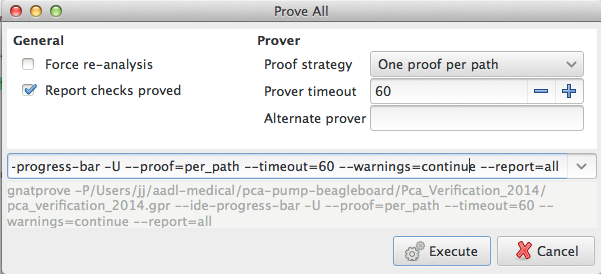
\includegraphics[width=0.7\textwidth]{figures/gnatprove-settings.png}        
    \end{center}
    \caption{GNATprove settings}
    \label{figure:gnatprove-settings}
\end{figure}

Summary of proof analysis is presented in the Figure \ref{listing:pca_pump_move_dosed_unit_spark2014_gnatprove}. Proof analysis returned three warnings: \lstinline{overflow check might fail} and one warning: \lstinline{contract case might fail}. It indicates the same problem like in verification with SPARK 2005 tools: potential for overflow. Additionally, there is a warning (\lstinline{postcondition might fail}) caused by tools limitations, which are not able to infer dependency between ghost function \lstinline{Dosed_State} and array \lstinline{Dosed}. If state refinement is not used (i.e. refined variables are defined in package specification), and actual array is used in the postcondition (instead of ghost function), this warning does not occur. The same program without abstract state is presented in the figures \ref{listing:pca_pump_move_dosed_unit_spark2014_no_refinement_spec} and \ref{listing:pca_pump_move_dosed_unit_spark2014_no_refinement_body}. Its verification summary is shown in the Figure \ref{listing:pca_pump_move_dosed_unit_spark2014_gnatprove_no_refinement}. 

%http://docs.adacore.com/spark2014-docs/html/ug/spark_2014.html#abstract-state-refined-state-and-initializes

\begin{figure}
\singlespacing
\begin{lstlisting}[frame=single, gobble=0]
analyzing Pca_Pump, 1 checks
analyzing Pca_Pump.Dosed_State, 0 checks
analyzing Pca_Pump.Dose_Volume_State, 0 checks
analyzing Pca_Pump.Sum, 3 checks
analyzing Pca_Pump.Read_Dosed, 4 checks
analyzing Pca_Pump.Increase_Dosed, 3 checks
analyzing Pca_Pump.Move_Dosed, 12 checks
pca_pump.adb:5:39: info: length check proved
pca_pump.adb:27:10: info: loop invariant initialization proved
pca_pump.adb:27:10: info: loop invariant preservation proved
pca_pump.adb:28:27: warning: overflow check might fail
pca_pump.adb:38:70: warning: overflow check might fail
pca_pump.adb:47:10: info: loop invariant initialization proved
pca_pump.adb:47:10: info: loop invariant preservation proved
pca_pump.adb:47:65: info: index check proved
pca_pump.adb:48:27: warning: overflow check might fail
pca_pump.adb:59:10: info: loop invariant initialization proved
pca_pump.adb:59:10: info: loop invariant preservation proved
pca_pump.adb:59:55: info: index check proved
pca_pump.ads:29:17: info: precondition proved
pca_pump.ads:29:48: info: overflow check proved
pca_pump.ads:36:14: warning: postcondition might fail, requires Dosed_State (Doses_Array_Index'Last) = 0
pca_pump.ads:37:6: info: disjoint contract cases proved
pca_pump.ads:37:6: info: complete contract cases proved
pca_pump.ads:37:66: warning: contract case might fail
pca_pump.ads:37:69: info: precondition proved
pca_pump.ads:37:86: info: precondition proved
pca_pump.ads:38:66: warning: contract case might fail
pca_pump.ads:38:69: info: precondition proved
pca_pump.ads:38:86: info: precondition proved
\end{lstlisting}
\doublespacing
\caption{GNATprove verification summary of module for dose monitoring in SPARK 2014}
\label{listing:pca_pump_move_dosed_unit_spark2014_gnatprove}
\end{figure}

\begin{figure}
\singlespacing
\begin{lstlisting}[language=ada2012, frame=single, gobble=0]
package Pca_Pump_No_Refinement
  with SPARK_Mode
is
   type Drug_Volume is range 0 .. 2**15-1;

   subtype Doses_Array_Index is Integer range 1 .. 60;
   type Doses_Array is array (Doses_Array_Index) of Drug_Volume;

   Dosed : Doses_Array := Doses_Array'(others => 0);
   Dose_Volume : Drug_Volume := 1;

   function Sum(Arr : Doses_Array) return Drug_Volume
     with Convention => Ghost;

   function Read_Dosed return Drug_Volume
     with Global  => (Input => (Dosed)),
     Pre     => Sum(Dosed) <= Drug_Volume'Last;

   procedure Increase_Dosed
     with Global  => (Input  => Dose_Volume, In_Out => Dosed),
     Depends => (Dosed => (Dosed, Dose_Volume)),
     Pre     => Read_Dosed <= Drug_Volume'Last - Dose_Volume;

   pragma Unevaluated_Use_Of_Old (Allow);

   procedure Move_Dosed
     with Global  => (In_Out => Dosed),
     Depends => (Dosed => Dosed),
     Post => (Dosed(Doses_Array_Index'Last) = 0),
     Contract_Cases => (Dosed(Doses_Array_Index'First) = 0 => Read_Dosed'Old = Read_Dosed,
                        Dosed(Doses_Array_Index'First) > 0 => Read_Dosed'Old > Read_Dosed);
end Pca_Pump_No_Refinement;
\end{lstlisting}
\doublespacing
\caption{Sequential module for dose monitoring in SPARK 2014 without variable refinement: package specification}
\label{listing:pca_pump_move_dosed_unit_spark2014_no_refinement_spec}
\end{figure}

\begin{figure}
\singlespacing
\begin{lstlisting}[language=ada2012, frame=single, gobble=0]
package body Pca_Pump_No_Refinement
  with SPARK_Mode
is
   function Sum(Arr : Doses_Array) return Drug_Volume
   is
      Result : Drug_Volume := 0;
   begin
      for I in Doses_Array_Index loop
         pragma Loop_Invariant (true);
         Result := Result + Arr(I);
      end loop;
      return Result;
   end Sum;

   procedure Increase_Dosed
   is
   begin
      Dosed(Doses_Array_Index'Last) := Dosed(Doses_Array_Index'Last) + Dose_Volume;
   end Increase_Dosed;

   function Read_Dosed return Drug_Volume
   is
      Result : Drug_Volume := 0;
   begin
      for I in Doses_Array_Index loop
         pragma Loop_Invariant (if I > 1 then Result >= Dosed (I-1));
         Result := Result + Dosed(I);
      end loop;
      return Result;
   end Read_Dosed;

   procedure Move_Dosed
   is
   begin
      for I in Doses_Array_Index range 1 .. Doses_Array_Index'Last-1 loop
         pragma Loop_Invariant (if I > 1 then Dosed (I-1) = Dosed (I));
         Dosed(I) := Dosed(I+1);
      end loop;
      Dosed(Doses_Array_Index'Last) := 0;
   end Move_Dosed;
end Pca_Pump_No_Refinement;
\end{lstlisting}
\doublespacing
\caption{Sequential module for dose monitoring in SPARK 2014 without variable refinement: package body}
\label{listing:pca_pump_move_dosed_unit_spark2014_no_refinement_body}
\end{figure}

\begin{figure}
\singlespacing
\begin{lstlisting}[frame=single, gobble=0]
analyzing Pca_Pump_No_Refinement, 1 checks
analyzing Pca_Pump_No_Refinement.Sum, 3 checks
analyzing Pca_Pump_No_Refinement.Read_Dosed, 4 checks
analyzing Pca_Pump_No_Refinement.Increase_Dosed, 3 checks
analyzing Pca_Pump_No_Refinement.Move_Dosed, 12 checks
pca_pump_no_refinement.adb:9:10: info: loop invariant initialization proved
pca_pump_no_refinement.adb:9:10: info: loop invariant preservation proved
pca_pump_no_refinement.adb:10:27: warning: overflow check might fail
pca_pump_no_refinement.adb:18:70: warning: overflow check might fail
pca_pump_no_refinement.adb:26:10: info: loop invariant initialization proved
pca_pump_no_refinement.adb:26:10: info: loop invariant preservation proved
pca_pump_no_refinement.adb:26:65: info: index check proved
pca_pump_no_refinement.adb:27:27: warning: overflow check might fail
pca_pump_no_refinement.adb:36:10: info: loop invariant initialization proved
pca_pump_no_refinement.adb:36:10: info: loop invariant preservation proved
pca_pump_no_refinement.adb:36:55: info: index check proved
pca_pump_no_refinement.ads:9:39: info: length check proved
pca_pump_no_refinement.ads:22:17: info: precondition proved
pca_pump_no_refinement.ads:22:48: info: overflow check proved
pca_pump_no_refinement.ads:29:14: info: postcondition proved
pca_pump_no_refinement.ads:30:6: info: disjoint contract cases proved
pca_pump_no_refinement.ads:30:6: info: complete contract cases proved
pca_pump_no_refinement.ads:30:60: warning: contract case might fail
pca_pump_no_refinement.ads:30:63: info: precondition proved
pca_pump_no_refinement.ads:30:80: info: precondition proved
pca_pump_no_refinement.ads:31:60: warning: contract case might fail
pca_pump_no_refinement.ads:31:63: info: precondition proved
pca_pump_no_refinement.ads:31:80: info: precondition proved
\end{lstlisting}
\doublespacing
\caption{GNATprove verification summary of module for dose monitoring in SPARK 2014 without variable refinement}
\label{listing:pca_pump_move_dosed_unit_spark2014_gnatprove_no_refinement}
\end{figure}


\section{Assessment}
\label{verification:assessment}

Verification presented in this chapter allowed to detect potentially dangerous run-time exceptions (e.g., overflow). In the future, it can be used also for verification of requirements specified by BLESS in AADL models. SPARK Examiner was helpful during implementation in flow errors detection, which indicates when package implementation does not conform to its specification.

